\documentclass{beamer}

\usepackage[utf8]{vietnam}

\usetheme{Warsaw}
\setbeamertemplate{frametitle continuation}{}

\title{Nhận diện bệnh trên cây cà phê\\ qua hình thái của lá}
\author{Nguyễn Quang Trường}
\institute{12 Toán - Trường THPT Chuyên Nguyễn Tất Thành}
\date{Kon Tum, \today}

\begin{document}

\frame{\titlepage}

\begin{frame}[allowframebreaks]{Lý do chọn đề tài}

	Kon Tum là một tỉnh thuộc khu vực Tây Nguyên, nổi tiếng với những loài cây công nghiệp lâu năm. Trong đó, cà phê có vai trò quan trọng đối với người dân nơi đây, đặc biệt là với đồng bào dân tộc thiểu số, giúp xóa đói, giảm nghèo, mang lại nguồn thu nhập lớn cho nhân dân tỉnh nhà.

	\framebreak

	Tuy nhiên, hằng năm, sâu bệnh trên cây cà phê đã gây thiệt hại nặng nề cho bà con và các doanh nghiệp sản xuất, chế biến cà phê bản địa.
	
	\framebreak
	
	Vì vậy, tác giả đã nghiên cứu và phát triển dự án: \textbf{Nhận diện một số sâu bệnh thường gặp trên cây cà phê qua hình thái của lá}.
	
	\null
	
	Đây là một hệ thống nhận diện thông minh, tương đối chính xác, nhằm giúp nhân dân, nhất là đồng bào dân tộc thiểu số nhận diện một số sâu bệnh thường gặp trên cây cà phê dễ dàng, thuận tiện để có các biện pháp phòng trừ sâu bệnh hiệu quả, góp phần cải thiện ngành trồng trọt cây cà phê tại tỉnh Kon Tum.

\end{frame}

\begin{frame}[allowframebreaks]{Câu hỏi nghiên cứu}

	Trước khi nghiên cứu, tác giả đưa ra một số câu hỏi nghiên cứu:
	
	\begin{itemize}
		\item Hiện tại, có những phương pháp nào để chẩn đoán bệnh trên cây cà phê? 
		\item Nhận dạng các đặc điểm của bệnh bằng mắt thường như thế nào? Làm thế nào để máy có thể nhận dạng tương tự? 
	\end{itemize}

	\framebreak

	Chẩn đoán thông qua đặc điểm hình thái được thể hiện trên lá
	\begin{itemize}
		\item Nhanh chóng, thuận tiện, chi phí thấp...
		\item Khó phát hiện các bệnh phức tạp, ít thể hiện trên hình thái
	\end{itemize}

	Phân tích cấu trúc lá trong phòng thí nghiệm:
	\begin{itemize}
		\item Độ chính xác cao, xác định được những bệnh phức tạp
		\item Nhiều thời gian, công sức phân tích, chi phí cơ sở vật chất...
	\end{itemize}

	\framebreak
	Với mong muốn xây dựng một giải pháp nhanh chóng và thuận tiện, phương pháp nghiên cứu thông qua đặc điểm hình thái là phương pháp được lựa chọn làm cơ sở cho việc xây dựng giải pháp.

	\framebreak

	Dự án nghiên cứu nhằm:

	\begin{itemize}
		\item Xây dựng một mô hình giúp nhân dân, đặc biệt là đồng bào dân tộc thiểu số (đa số có trình độ dân trí thấp, chưa biết ứng dụng khoa học kĩ thuật vào canh tác) nhận diện các loại sâu bệnh trên cây cà phê qua hình ảnh với độ chính xác cao;
		\item Ứng dụng mô hình vào thực tiễn tại địa phương, giúp giảm thiểu thiệt hại do sâu bệnh gây ra, góp phần phát triển kinh tế - xã hội trên địa bàn, giúp đồng bào dân tộc thiểu số vươn lên thoát nghèo, làm giàu trên chính quê hương của mình.
	\end{itemize}

\end{frame}

\begin{frame}[allowframebreaks]{Ý nghĩa của dự án}
	
	Ý nghĩa khoa học:

	\null

	$\bullet$ Đề tài nghiên cứu phương pháp nhận diện qua hình ảnh, tuy phổ biến trên những đối tượng khác, nhưng lại ít được quan tâm trên cây cà phê.
	
	\null

	$\Rightarrow$ Mở rộng nghiên cứu nhận diện hình ảnh trên cây cà phê sau này.

	\framebreak

	Ý nghĩa xã hội:

	\null

	$\bullet$ Đối tượng nghiên cứu của dự án là cây cà phê, một trong những cây công nghiệp quan trọng ở tỉnh Kon Tum.

	\null

	$\Rightarrow$ Hướng đến giúp đỡ nhân dân, đặc biệt là đồng bào dân tộc thiểu số dễ dàng nhận diện một số sâu bệnh cơ bản để có cách phòng trừ hiệu quả, góp phần xóa đói, giảm nghèo, phát triển kinh tế - xã hội trên địa bàn.

\end{frame}

\begin{frame}[allowframebreaks]{Dữ liệu}

	Dữ liệu được kết hợp thu thập từ thực địa, và từ các tập dữ liệu khác trên mạng.
	
	\null
	
	Dữ liệu từ thực địa được thu thập tại huyện Đăk Hà (huyện nổi tiếng về sản xuất cà phê trên địa bàn tỉnh Kon Tum) và xã Ia Chim (xã trồng nhiều cây cà phê của thành phố Kon Tum).

	\framebreak

	\begin{itemize}
		\item Bộ dữ liệu gồm 1747 bức ảnh chụp các lá cà phê chè (bao gồm lá bình thường, và lá bị một hoặc nhiều bệnh)
		\item Sau tiền xử lý, thu được 2722 bức ảnh cắt xung quanh vùng có bệnh và không có bệnh trên lá
		\item Được chia ra thành 3 tập con tách biệt: training set, validation set và test set, theo tỉ lệ 70-15-15.
	\end{itemize}

	\framebreak

	\begin{figure}[H]
		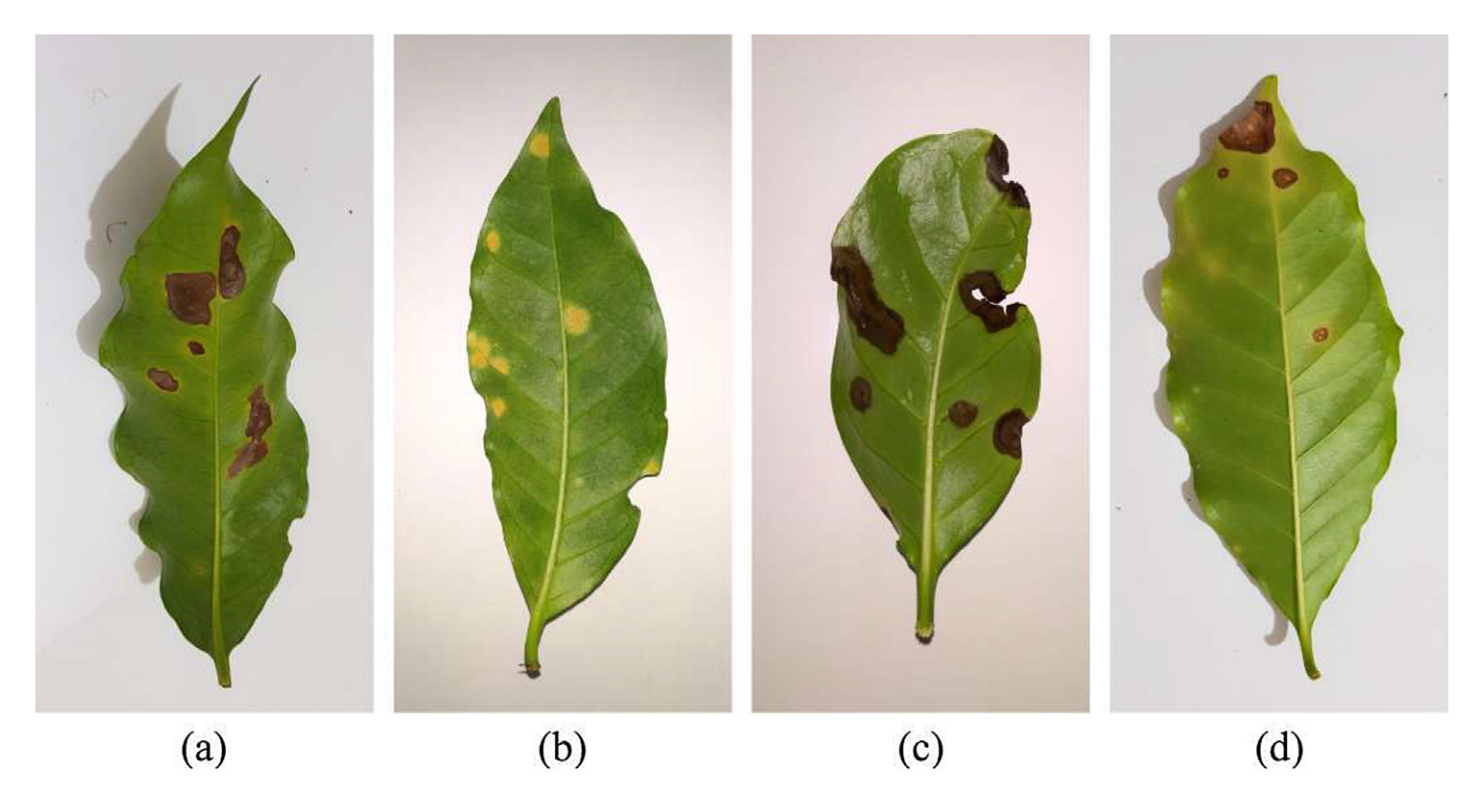
\includegraphics[scale=0.25]{images/image1}
		\caption{Các bệnh: sâu vẽ bùa (a), gỉ sắt (b), đốm nâu (c), đốm mắt cua (d)}
	\end{figure}

	\framebreak
	% \framebreak
	
	\begin{figure}[H]
		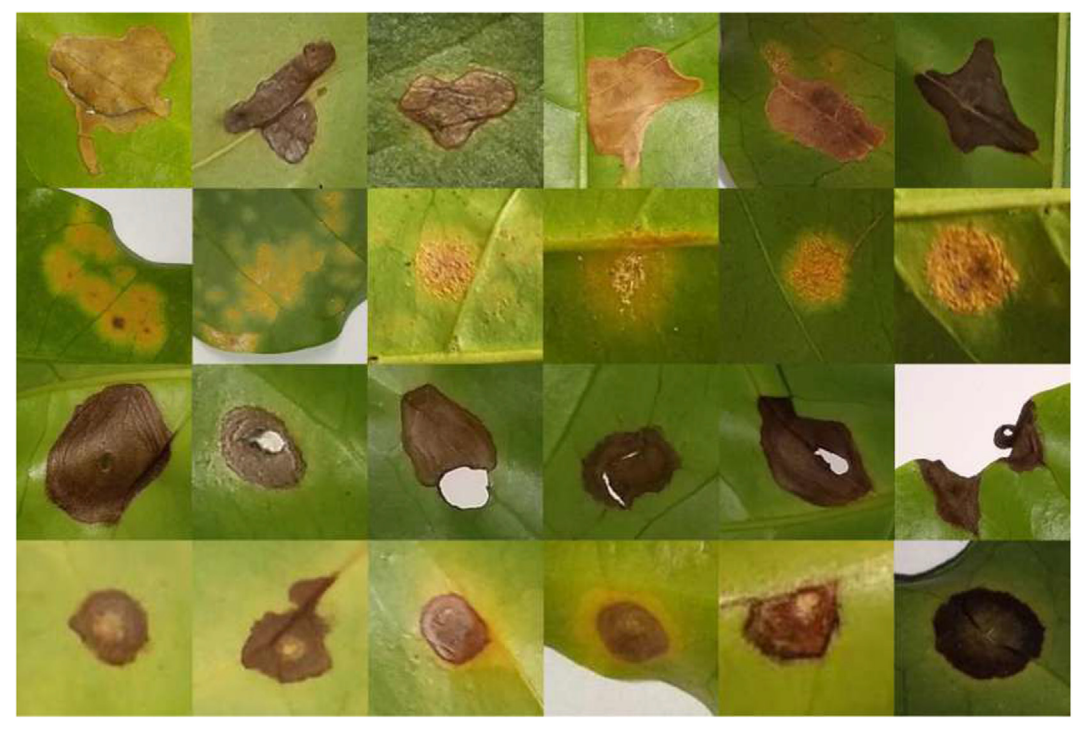
\includegraphics[scale=0.35]{images/image3}
		\caption{Các vùng được cắt sau tiền xử lý}
	\end{figure}

	\framebreak

	\begin{table}[]
		\begin{tabular}{|c|c|}
		\hline
		Bệnh        & Số lượng ảnh \\ \hline
		Bình thường & 256          \\
		Sâu vẽ bùa  & 593          \\
		Gỉ sắt      & 991          \\
		Đốm nâu     & 504          \\
		Đốm mắt cua & 378          \\ \hline
		Tổng        & 2722         \\ \hline
		\end{tabular}

		\caption{Thống kê dữ liệu sau tiền xử lý}
	\end{table}


	\framebreak
	Trên thực tế, để rèn luyện cho một mô hình phức tạp, số lượng ảnh thu thập được như trên vẫn chưa đảm bảo, dễ dẫn đến tình trạng overfitting.

	\framebreak

	Data Augmentation: lấy những dữ liệu đã có sẵn, chỉnh sửa để tạo ra những dữ liệu mới, mà không làm mất đi tính chất tổng quát của ảnh.

	\begin{figure}[H]
		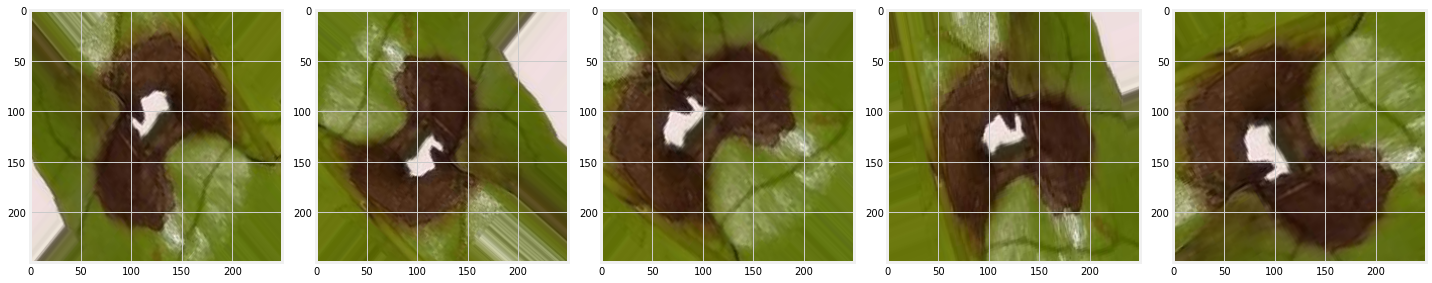
\includegraphics[scale=0.2]{images/image2}
		\caption{Ảnh được chỉnh sửa trong bước Data Augmentation}
	\end{figure}

\end{frame}

\begin{frame}[allowframebreaks]{Mô hình}
	Bằng việc xây dựng một mạng lưới mô phỏng hoạt động của các nơ-ron thần kinh trong não bộ con người, một chiếc máy cũng có thể tự học và dự đoán được các loại sâu bệnh khác nhau. Đây chính là nền tảng của Deep Learning, một nhánh con của Trí tuệ Nhân tạo.

	\begin{figure}[H]
		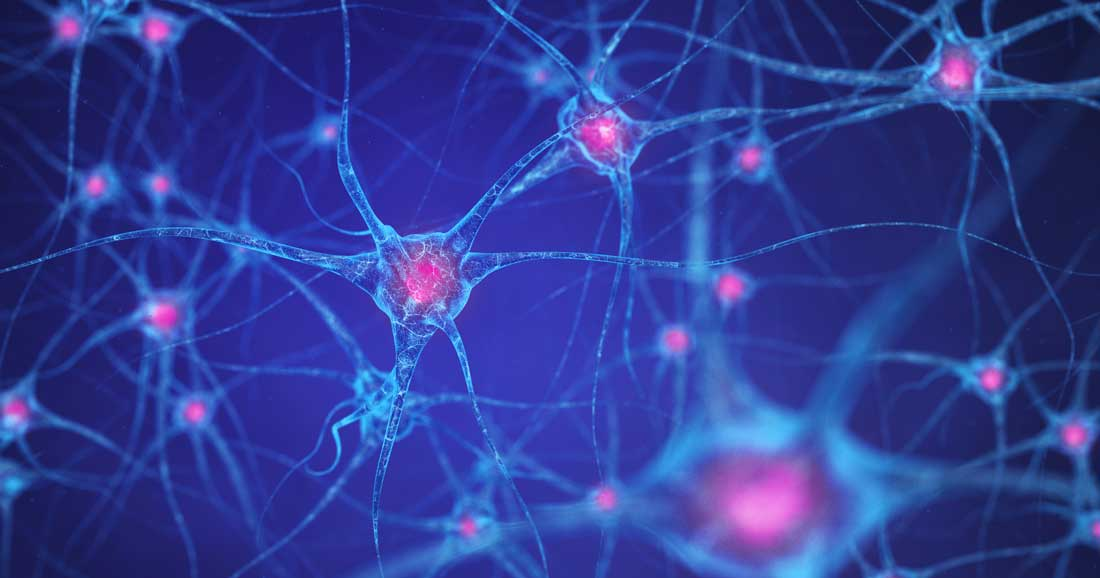
\includegraphics[scale=0.5]{images/image10}
		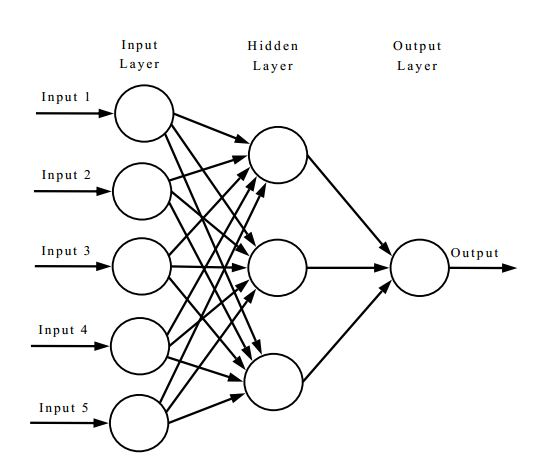
\includegraphics[scale=0.2]{images/image15}
		\caption{Nơ-ron của người (trái) và Mạng nơ-ron (phải)}
	\end{figure}

	\framebreak

	Các mô hình được thử nghiệm trong dự án bao gồm: InceptionV3, MobileNetV2, ResNet50V2, VGG16 và Xception. Những mô hình này đều đã được học qua ImageNet và được tiếp tục luyện trên toàn bộ mạng bằng dữ liệu mới mà không đóng băng bất cứ thông số nào.

	\framebreak

	\begin{table}[H]
		\centering
		\begin{tabular}{|c|c|c|}
		\hline
		Kiến trúc   & Số lượng tham số (triệu) & Số tầng \\ \hline
		InceptionV3 & 24                       & 48      \\
		MobileNetV2 & 2,2                      & 54      \\
		ResNet50V2  & 25                       & 50      \\
		VGG16       & 138                      & 16      \\
		Xception    & 23                       & 71      \\ \hline
		\end{tabular}

		\caption{Thông số của các kiến trúc được thử nghiệm}
	\end{table}

	\framebreak
	Các Siêu Tham số (Hyperparameter) được sử dụng cho các mô hình bao gồm:

	\begin{itemize}
		\item Batch size: 24
		\item Epochs: 50
		\item Hàm mất mát: Categorical Cross-Entropy
		\item Hàm tối ưu: Stochastic Gradient Descent
			($\alpha$ = 0.001,\\$\eta$ = 0.9)
		\item Hàm tiêu biến: L2 Regularization ($\lambda = 5 \times 10^{-4}$)
	\end{itemize}

	\framebreak

	Các mô hình được huấn luyện trên môi trường Google Colab (GPU NVIDIA Tesla K80). Thư viện Keras được sử dụng để xây dựng và huấn luyện cho mô hình.

	\framebreak

	\begin{figure}[H]
		\centering
		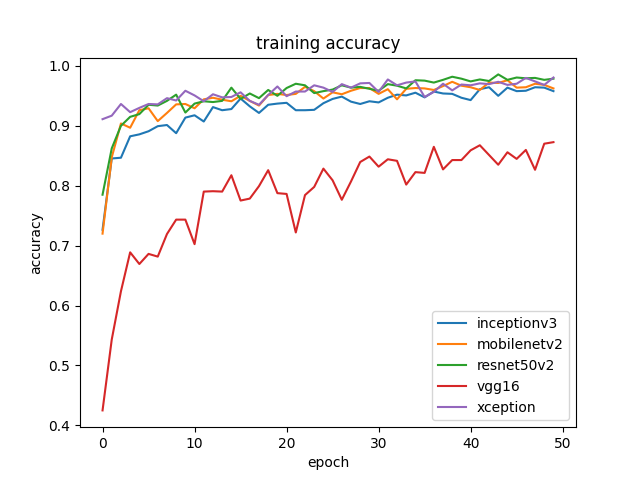
\includegraphics[scale=0.32]{images/accuracy.png}
		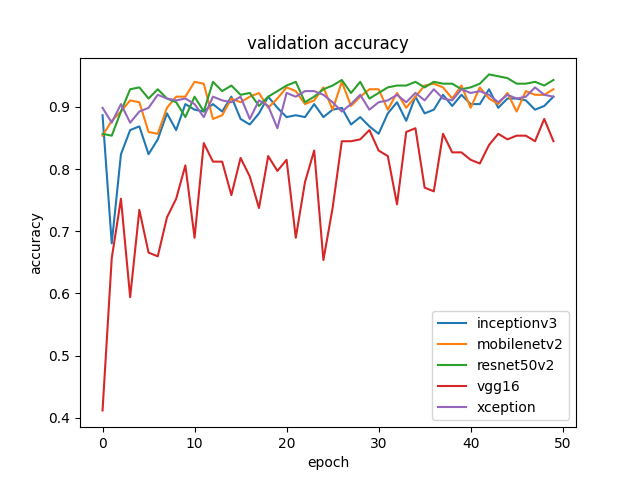
\includegraphics[scale=0.32]{images/val_accuracy.png}
		\caption{Biểu đồ accuracy trên training set và validation set}
	\end{figure}

	\framebreak

	\begin{figure}[H]
		\centering
		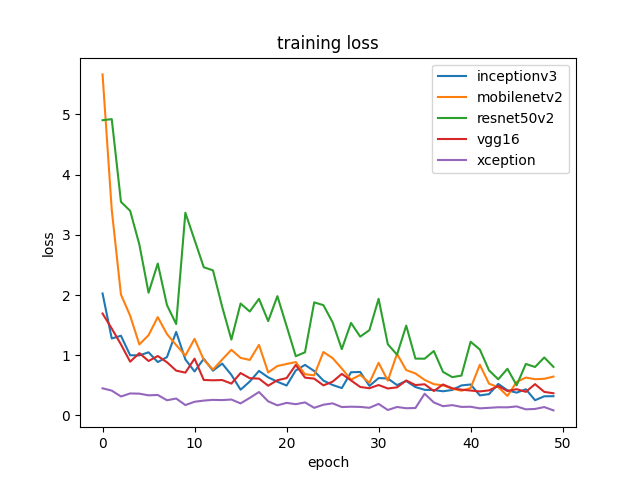
\includegraphics[scale=0.32]{images/loss.png}
		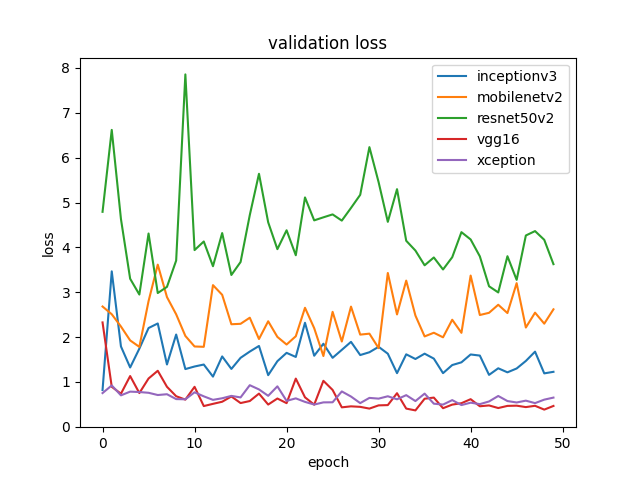
\includegraphics[scale=0.32]{images/val_loss.png}
		\caption{Biểu đồ loss trên training set và validation set}
	\end{figure}

	\framebreak

	\begin{table}[H]
		\centering
		\begin{tabular}{|c|c|c|c|}
			\hline
			Kiến trúc   & Accuracy (\%) & Precision (\%) & Recall (\%) \\ \hline
			InceptionV3 & \textbf{93}   & \textbf{93}    & \textbf{93} \\
			MobileNetV2 & 90            & 90             & 90          \\
			ResNet50v2  & \textbf{93}   & \textbf{93}    & \textbf{93} \\
			VGG16       & 84            & 84             & 84          \\
			Xception    & \textbf{93}   & \textbf{93}    & \textbf{93} \\ \hline
		\end{tabular}
		\caption{Kết quả đo các mô hình trên test set}
	\end{table}

	\framebreak

	Ba mô hình InceptionV3, ResNet50V2 và Xception đều có kết quả đo tương đương: 93\% trên cả Accuracy, Precision và Recall, vượt trội so với MobileNetV2 và VGG16.
	
	\null

	Dựa trên các biểu đồ khi huấn luyện, Xception có tốc độ học nhanh và chính xác, InceptionV3 không thua kém quá nhiều, còn ResNet50V2 không ổn định trong suốt quá trình học.

	\framebreak

	\begin{figure}[H]
		\centering
		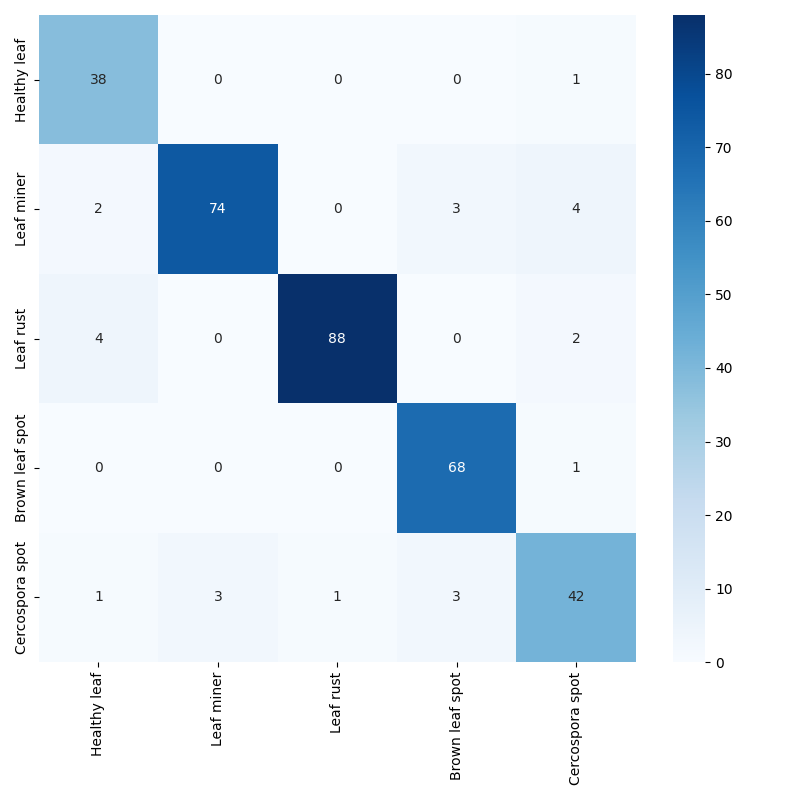
\includegraphics[scale=0.3]{images/xception_matrix.png}
		\caption{Confusion Matrix của Xception}
	\end{figure}

	\framebreak

	Sau quá trình nghiên cứu và thử nghiệm, mô hình \textbf{Xception} là mô hình phù hợp nhất với bài toán. Mô hình này là một Mạng Nơ-ron Tích chập (Convolutional Neural Network), thường được sử dụng cho các bài toán phân loại, với ưu điểm là gọn nhẹ, tính toán nhanh mà vẫn đảm bảo độ chính xác.

	\framebreak

	\begin{figure}[H]
		\centering
		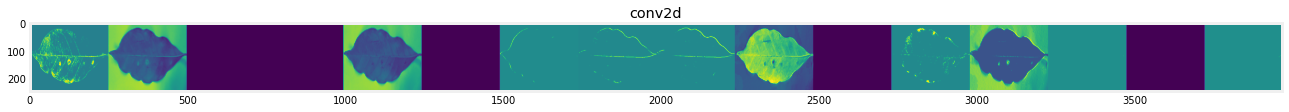
\includegraphics[scale=0.2]{images/image5}
		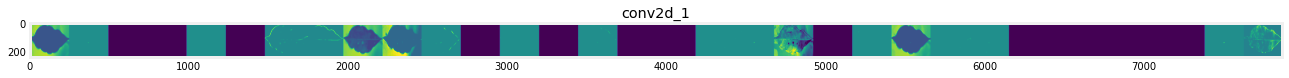
\includegraphics[scale=0.2]{images/image6}
		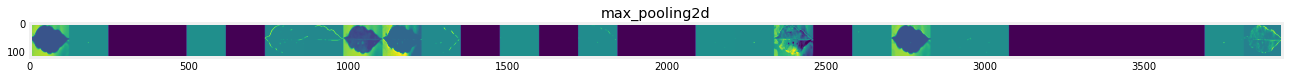
\includegraphics[scale=0.2]{images/image4}
		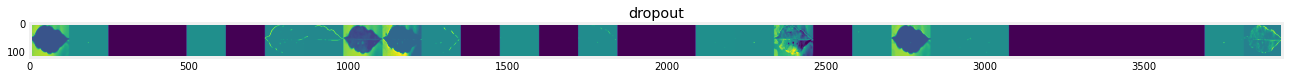
\includegraphics[scale=0.2]{images/image8}
		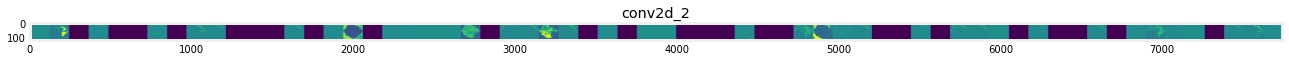
\includegraphics[scale=0.2]{images/image12}
		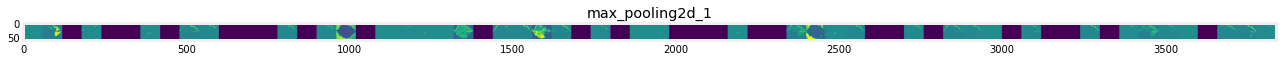
\includegraphics[scale=0.2]{images/image14}
		\caption{Kết quả xử lý của các nơ-ron của một vài tầng}
	\end{figure}

\end{frame}

\begin{frame}[allowframebreaks]{Ứng dụng}
	
	Để ứng dụng kết quả từ mô hình trên vào thực tế, tác giả đã phát triển một ứng dụng di động, liên lạc với máy chủ để xử lý.

	\framebreak

	\begin{figure}[H]
		\centering
		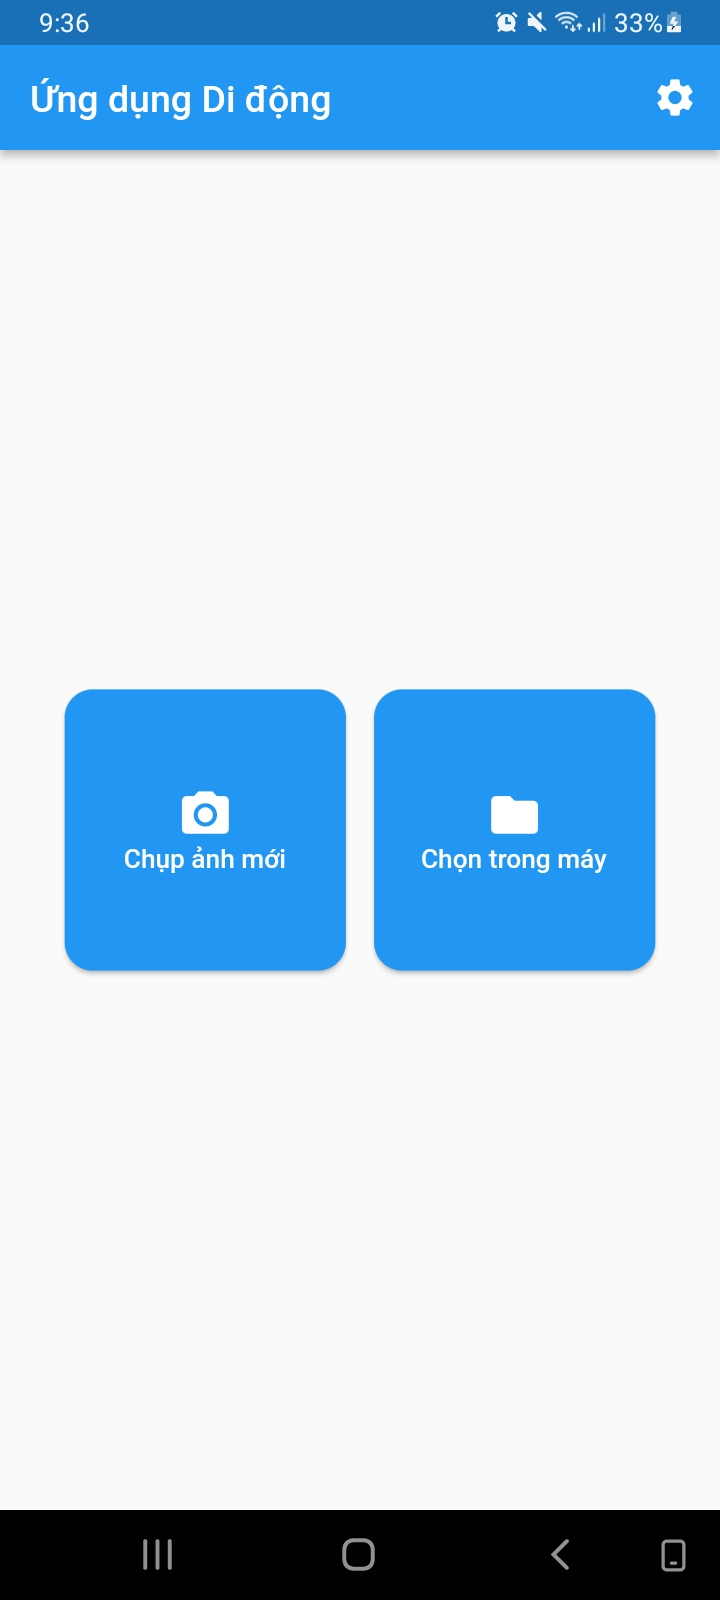
\includegraphics[scale=0.1]{images/screenshot1.jpg}
		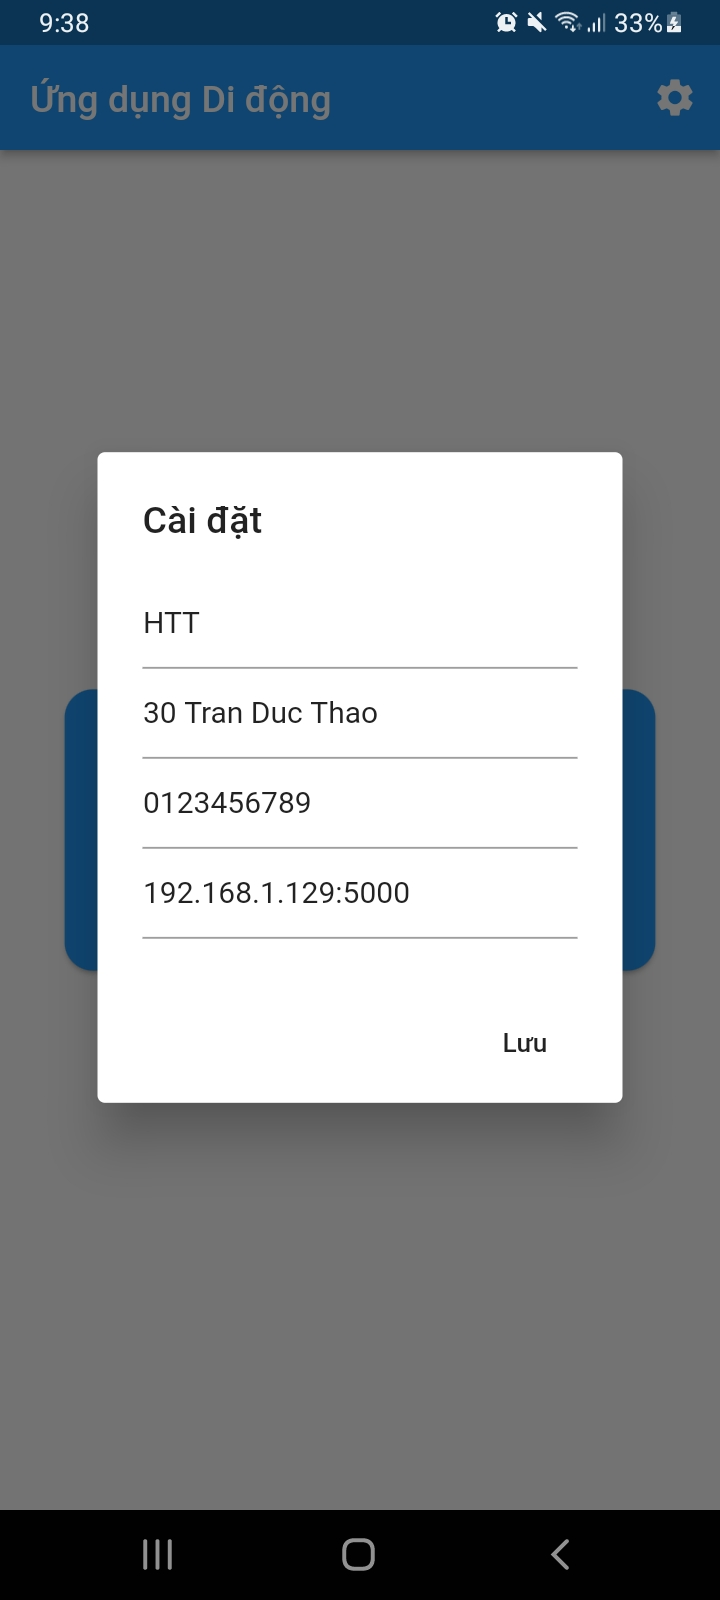
\includegraphics[scale=0.1]{images/screenshot2.jpg}
		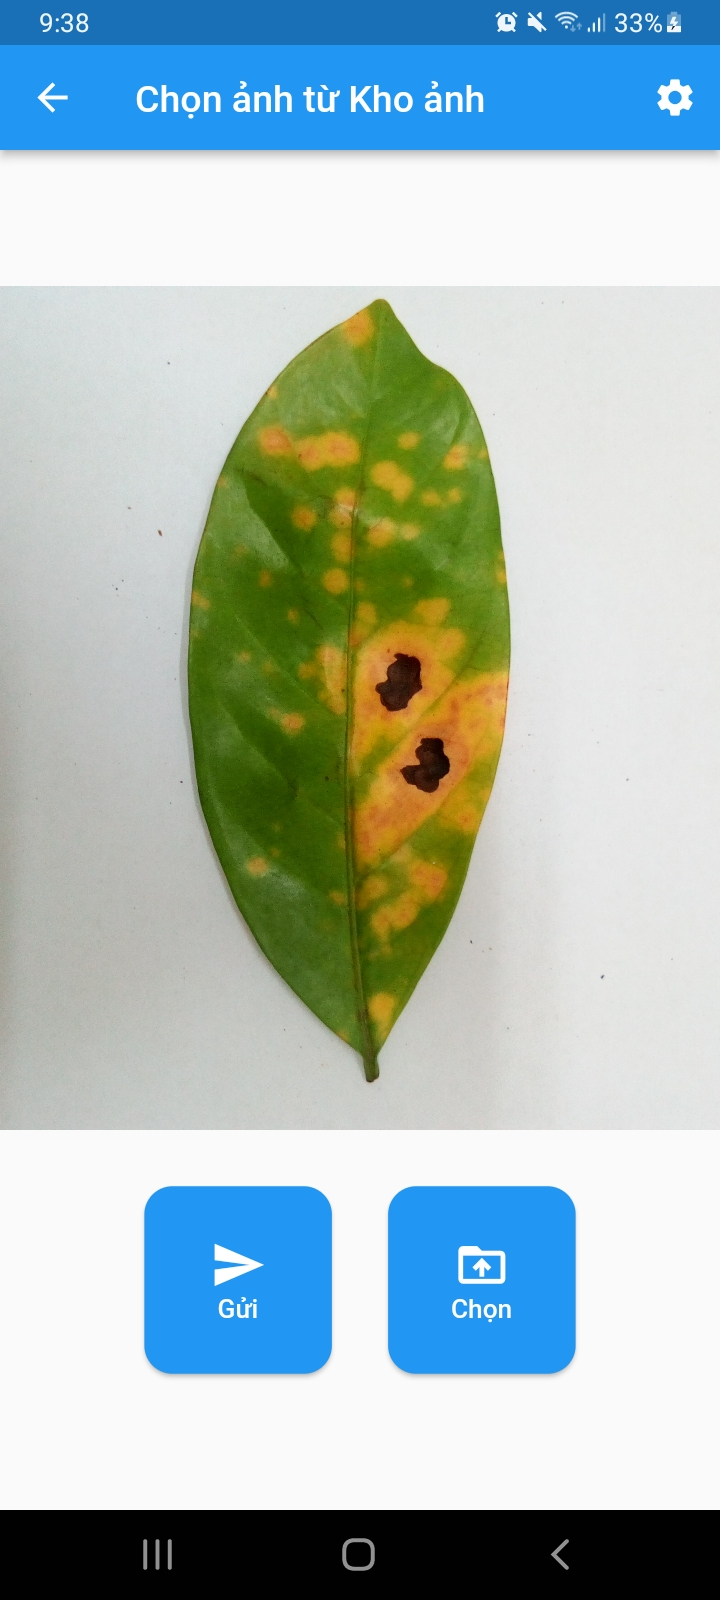
\includegraphics[scale=0.1]{images/screenshot3.jpg}
		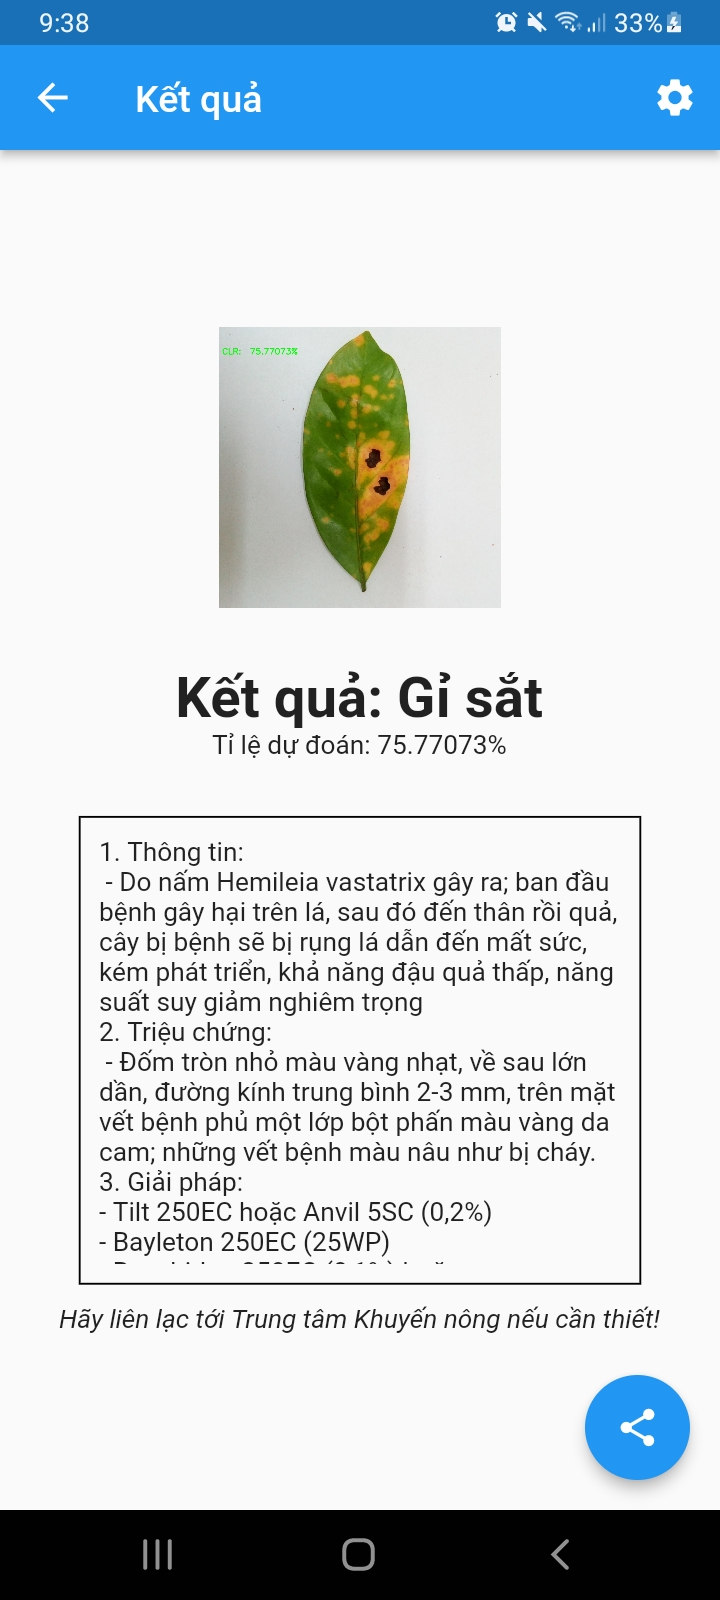
\includegraphics[scale=0.1]{images/screenshot4.jpg}
		\caption{Giao diện của ứng dụng di động}
	\end{figure}

	\framebreak

	Ứng dụng được thiết kế đơn giản, gọn nhẹ, dễ sử dụng với bà con, đặc biệt là đồng bào dân tộc thiểu số.

	\null

	Ứng dụng cho phép người dùng gửi hình ảnh (ảnh có sẵn trong máy hoặc ảnh chụp mới) lên máy chủ. Máy chủ tiếp nhận ảnh, xử lý ảnh bằng mô hình được xây dựng, rồi trả kết quả chẩn đoán về lại ứng dụng. Các kết quả trả về bao gồm tên bệnh, một số triệu chứng, đặc điểm đặc trưng và tên một vài thuốc đặc trị cho sâu bệnh.

	\framebreak

	\begin{figure}[H]
		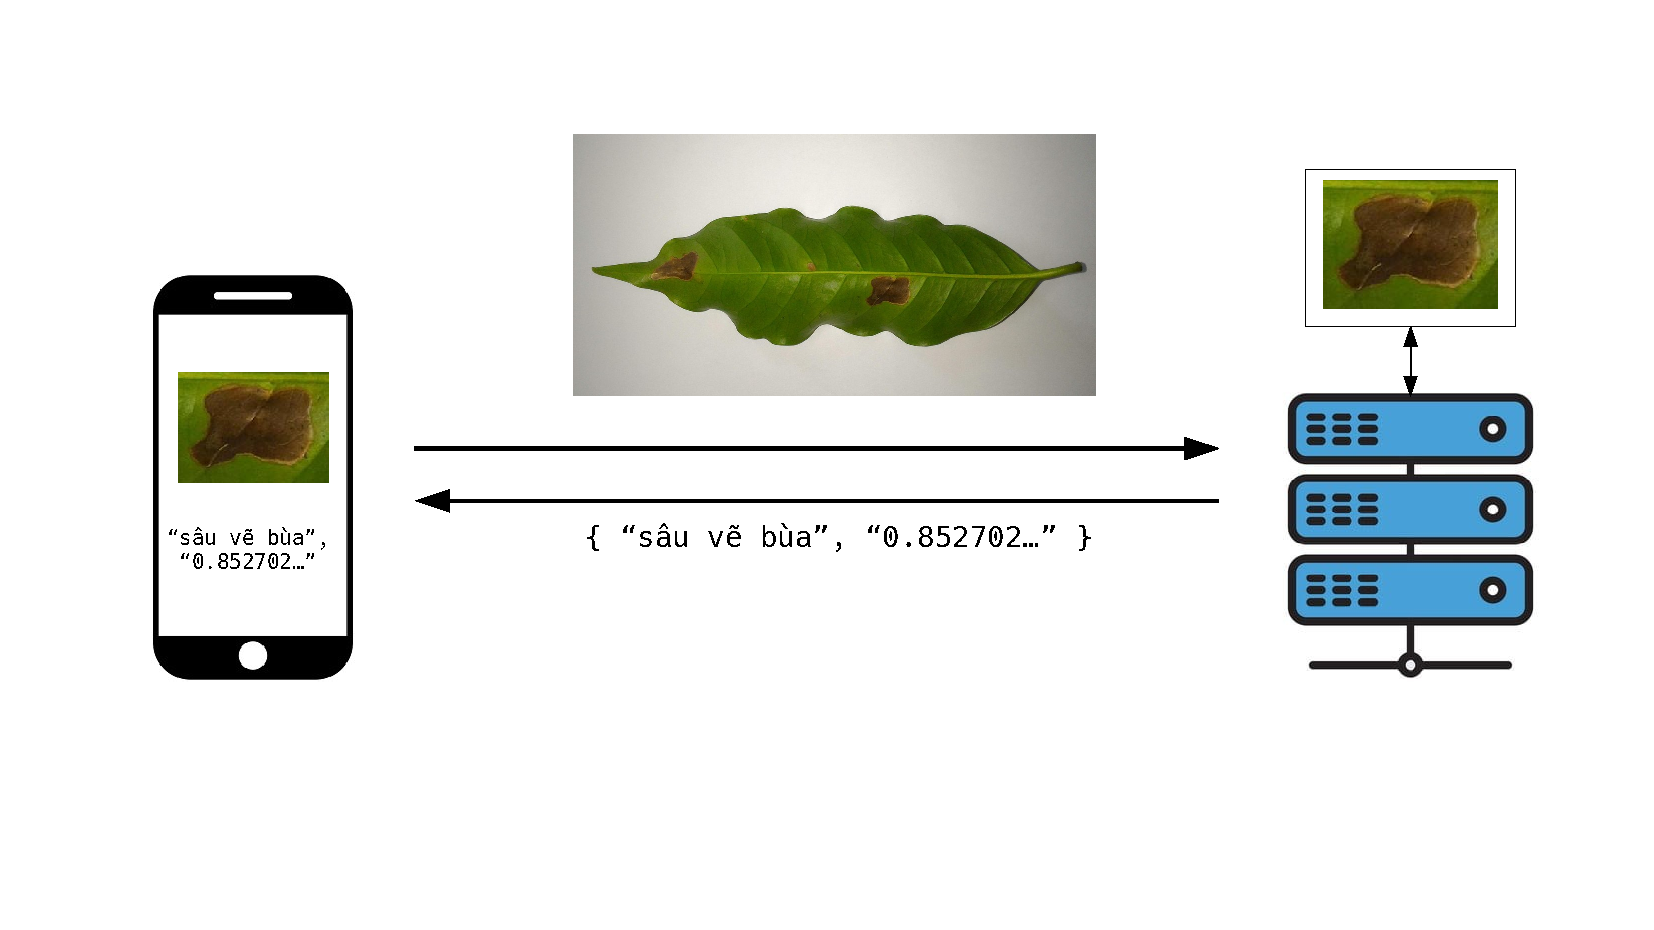
\includegraphics[scale=0.35]{images/chart.pdf}
		\caption{Sơ đồ hoạt động}
	\end{figure}

\end{frame}

\begin{frame}[allowframebreaks]{Kết luận}
	Trí tuệ Nhân tạo là một phương pháp khả thi để nhận diện sâu bệnh qua hình thái của lá cà phê, và hoàn toàn có thể tiếp tục phát triển trong tương lai, mở rộng sang nhiều giống cây trồng khác, phục vụ người nông dân ở khắp mọi miền đất nước.

	\framebreak

	Ưu điểm:
	\begin{itemize}
		\item Tỉ lệ nhận diện mang lại hiệu quả tương đối chính xác;
		\item Tiết kiệm thời gian, công sức, chi phí cho việc chẩn đoán so với các phương pháp hiện có;
		\item Ứng dụng di động gọn nhẹ, đơn giản, dễ sử dụng.
	\end{itemize}

	\framebreak

	Nhược điểm:
	\begin{itemize}
		\item Mô hình vẫn chưa thực sự tối ưu, quá trình rèn luyện chưa đạt kết quả tốt nhất, tốc độ nhận diện còn chậm;
		\item Kích thước tập dữ liệu để rèn luyện còn hạn chế, cần được mở rộng và làm phong phú thêm;
		\item Cần bổ sung thêm cơ sở dữ liệu về sâu bệnh và các thông tin liên quan.
	\end{itemize}

	\framebreak

	Hướng phát triển 
	\begin{itemize}
		\item Cải tiến mô hình, cải tiến phương pháp luyện để khai thác hết tiềm năng của mô hình, thử nghiệm với những mô hình mới;
		\item Thu thập thêm dữ liệu, xây dựng một bộ cơ sở dữ liệu trung tâm;
		\item Hoàn thiện, phát triển thêm tính năng cho ứng dụng di động;
		\item Hợp tác với các nhà nghiên cứu về cây cà phê để tiếp tục hoàn thiện dự án.
	\end{itemize}

\end{frame}

\begin{frame}
	\centering \Large
	Cảm ơn.
\end{frame}

\end{document}